\chapter{Implementacija i korisničko sučelje}
		
		
		\section{Korištene tehnologije i alati}
	
			
\textbf{	KORIŠTENE TEHNOLOGIJE
} 

Prilikom izrade web aplikacija za upravljanje rehabilitacijom koristili smo razne tehnologije kako bismo pružili korisnicima učinkovit i interaktivan doživljaj. \textit{Backend} aplikacije razvili smo koristeći \href{https://www.spring.io/projects/spring-boot}{Spring Boot}, \href{https://www.oracle.com/java}{Java} bazirani okvir, koji omogućava brz i jednostavan razvoj logike sa serverske strane. \href{https://www.oracle.com/java}{Java} doprinosi robustnosti i skalabilnosti našeg \textit{backend} sustava.

Za dinamičke i interaktivne elemente na korisničkom sučelju, koristili smo \href{https://www.developer.mozilla.org/en-US/docs/Web/JavaScript}{JavaScript}, dok je \href{https://www.reactjs.org}{React}, popularni \href{https://www.developer.mozilla.org/en-US/docs/Web/JavaScript}{JavaScript} okvir, omogućio izgradnju efikasnog korisničkog sučelja. \href{https://www.reactjs.org}{React}, koristeći koncept komponenti, pojednostavljuje organizaciju i održavanje koda, pridonoseći poboljšanju korisničkog iskustva i olakšavajući upravljanje stanjem naše aplikacije.

Podaci o pacijentima, terapijama i terminima pohranjeni su u \href{https://www.postgresql.org}{PostgreSQL} bazi podataka koja pruža pouzdanu podršku. \href{https://www.postgresql.org}{PostgreSQL}, kao snažan objektno-relacijski sustav upravljanja bazama podataka, omogućava nam efikasno upravljanje informacijama uz podršku za kompleksne upite i transakcije. Osim toga, \href{https://www.developer.mozilla.org/en-US/docs/Web/HTML}{HTML} i \href{https://www.developer.mozilla.org/en-US/docs/Web/CSS}{CSS} koriste se za strukturiranje sadržaja web stranice i stilizaciju, stvarajući tako funkcionalno i atraktivno korisničko sučelje.

Dokumentacija projekta oblikovana je pomoću \href{https://www.overleaf.com/learn/latex/Learn_LaTeX_in_30_minutes}{LaTeX} sustava za pripremu dokumenata, pružajući precizno formatiranje i organizaciju. Za organizaciju sastanaka i suradnju koristili smo \href{https://www.markdownguide.org}{Markdown} format, pružajući jednostavan i čitljiv način za pisanje i dijeljenje informacija.

U procesu zajedničkog rada, pisanja koda i praćenja promjena koristili smo \href{https://git-scm.com/}{Git}. Omogućavao je stvaranje, pregledavanje i spajanje promjena koda, čime se postizavao učinkovit timski rad. Sve ove tehnologije integrirane su u našem projektu kako bismo osigurali da interakcija između bolesnika, djelatnika zdravstvene ustanove i administratora bude glatka, učinkovita i prilagođena specifičnim ulogama i funkcionalnim zahtjevima svakog dionika.

Python je bio ključan u razvoju našeg AI chat bota, iskoristili smo njegove sposobnosti u strojnom učenju i obradi prirodnog jezika za stvaranje interaktivnog i inteligentnog sučelja za korisnike. Python smo još koristili u kombinaciji sa Selenium WebDriverom za automatizaciju testiranja korisničkog sučelja, omogućavajući simulaciju stvarnih interakcija korisnika i osiguravajući pouzdanost naše web aplikacije.

\textbf{KORIŠTENI ALATI
}

U procesu razvoja naše aplikacije koristili smo raznovrsne alate kako bismo unaprijedili različite aspekte projekta. Alat \href{https://www.heroku.com}{Heroku}, poznat po svojoj \textit{cloud} platformi, omogućio nam je jednostavno postavljanje, skaliranje i učinkovito upravljanje web aplikacijama. Korištenjem \href{https://www.heroku.com}{Heroku}-a, značajno smo pojednostavili proces implementacije i održavanja naše aplikacije.

Za potrebe pisanja, testiranja i ispravljanja koda koristili smo \href{https://www.visualstudio.com}{Visual Studio Code} (\href{https://www.visualstudio.com}{VSCode}), integrirano razvojno okruženje (IDE). \href{https://www.visualstudio.com}{VSCode} pružio je alate koji su povećali efikasnost našeg tima tijekom razvoja aplikacije. \href{https://www.jetbrains.com/idea}{IntelliJ IDEA}, kao razvojno okruženje specifično za Java programski jezik, optimizirao je rad na \textit{backend} dijelu naše aplikacije. 

\href{https://github.com}{GitHub}, platforma za upravljanje verzijama koda i suradnju timova, poslužila nam je za praćenje promjena, upravljanje zadacima te implementaciju \textit{pull requestova}, unapređujući suradnju tima. Za brzu i jednostavnu komunikaciju te video razgovore koristili smo \href{https://discord.com}{Discord}, pružajući središnje mjesto za razmjenu informacija između članova tima.


\href{https://www.notion.so}{Notion}, kao alat za organizaciju zadataka, vođenje bilješki sastanaka i općenito upravljanje projektom, korišten je kako bi pridonio boljoj organizaciji i praćenju napretka. \href{https://www.overleaf.com}{Overleaf}, online platforma za suradničko pisanje dokumenata u LaTeX formatu, olakšala je stvaranje i uređivanje dokumentacije našeg projekta.
\href{https://www.visual-paradigm.com}{Visual Paradigm} pruža alate za izradu različitih dijagrama, a mi smo ga koristili za izradu dijagrama obrasca uporabe, sekvencijskih dijagrama, dijagrama stanja, aktivnosti i komponenata potrebnih za dokumentaciju. 

\href{https://www.figma.com}{Figma}, alat za dizajn, poslužio nam je u izradi vizualnih planova naše web aplikacije. Kroz Figmu definirali smo izgled \textit{frontend} dijela naše aplikacije. \href{https://www.adobe.com/products/premiere.html}{Adobe Premiere Pro} i \href{https://www.adobe.com/products/audition.html}{Audition} koristili smo za video i audio produkciju, stvarajući marketinške materijale i prezentacije vezane uz našu aplikaciju.

Naša interakcija s \href{https://openai.com/gpt}{ChatGPT}om bila je višestruko korisna, pružajući podršku u različitim aspektima, uključujući punjenje baze podataka te pružanje informacija i savjeta za vrijeme razvoja projekta. 


 		Napomena: Prilikom klika u tekstu na nazive korištenih alata i tehnologija otvara se internet poveznica na kojoj se može saznati više informacija o njima. Unatoč tome ovdje su navedene internet poveznice na kojima je moguće saznati više:  https://www.spring.io/projects/spring-boot, https://www.oracle.com/java,  https://www.developer.mozilla.org/en-US/docs/Web/JavaScript, https://www.reactjs.org, https://www.postgresql.org, https://www.developer.mozilla.org/en-US/docs/Web/HTML, https://www.developer.mozilla.org/en-US/docs/Web/CSS, https://www.overleaf.com/learn/latex,  https://www.markdownguide.org, https://git-scm.com, https://www.heroku.com, https://www.visualstudio.com, https://www.jetbrains.com/idea, https://github.com, https://discord.com, https://www.notion.so, https://www.overleaf.com, https://www.visual-paradigm.com, https://www.figma.com, https://www.adobe.com/products/premiere.html, https://www.adobe.com/products/audition.html, https://openai.com/gpt
			\eject 
		
	
			\section{Ispitivanje programskog rješenja}
			
			Ispitivanje komponenti provedeno je na razredima  \href{https://github.com/Project-MedBay/backend/blob/main/src/test/java/com/medbay/TherapyTypeServiceTest.java}{TherapyTypeService} 
			i \href{https://github.com/Project-MedBay/backend/blob/main/src/test/java/com/medbay/TherapyServiceTest.java}{TherapyService} u okruženju \texttt{com.medbay}. Slijede rezultati pojedinih ispitnih slučajeva:
			\newline \textbf{Rezultati ispitivanja komponenti za \href{https://github.com/Project-MedBay/backend/blob/main/src/test/java/com/medbay/TherapyTypeServiceTest.java}{TherapyTypeService}}

			\begin{enumerate}
				\item \textbf{Test: getTherapyType\_ReturnsListOfTherapyTypes}
				\begin{itemize}
					\item \textit{Opis:} Provjera vraćanja liste tipova terapija.
					\item \textit{Rezultat:} Test uspješan. Vraćena lista tipova terapija.
				\end{itemize}
\begin{lstlisting}[language=Java]
@Test
void getTherapyType_ReturnsListOfTherapyTypes() {
	List<TherapyType> expectedTherapyTypes = Arrays.asList(buildTherapyType("1"), buildTherapyType("2"));
	when(therapyTypeRepository.findAll()).thenReturn(expectedTherapyTypes);
	ResponseEntity<List<TherapyType>> response = therapyTypeService.getTherapyType();
	assertEquals(HttpStatus.OK, response.getStatusCode());
	assertEquals(expectedTherapyTypes, response.getBody());
	}
\end{lstlisting}

				\item \textbf{Test: getTherapyType\_WhenNoTherapyTypes\_ReturnsEmptyList}
				\begin{itemize}
					\item \textit{Opis:} Provjera vraćanja prazne liste kada nema tipova terapija.
					\item \textit{Rezultat:} Test uspješan. Vraćena prazna lista.
				\end{itemize}
\begin{lstlisting}[language=Java]
@Test
void getTherapyType_WhenNoTherapyTypes_ReturnsEmptyList() {
	when(therapyTypeRepository.findAll()).thenReturn(Collections.emptyList());
	ResponseEntity<List<TherapyType>> response = therapyTypeService.getTherapyType();
	assertEquals(HttpStatus.OK, response.getStatusCode());
	assertTrue(Objects.requireNonNull(response.getBody()).isEmpty());
		}
\end{lstlisting}

				\item \textbf{Test: getTherapyType\_WhenRepositoryThrowsException\_ReturnsErrorResponse}
				\begin{itemize}
					\item \textit{Opis:} Provjera odziva na iznimku iz repozitorija.
					\item \textit{Rezultat:} Test uspješan. Izazvana iznimka.
				\end{itemize}

\begin{lstlisting}[language=Java]
@Test
void getTherapyType_WhenRepositoryThrowsException_ReturnsErrorResponse() {
	when(therapyTypeRepository.findAll()).thenThrow(new RuntimeException("Database error"));
	assertThrows(RuntimeException.class, () -> therapyTypeService.getTherapyType());
}
\end{lstlisting}
			\end{enumerate}
			
			Svi ispitni slučajevi su prošli uspješno, što ukazuje na pouzdanost i stabilnost implementiranih funkcionalnosti u razredu \texttt{TherapyTypeService}. 
			\begin{figure}[h]
				\centering
				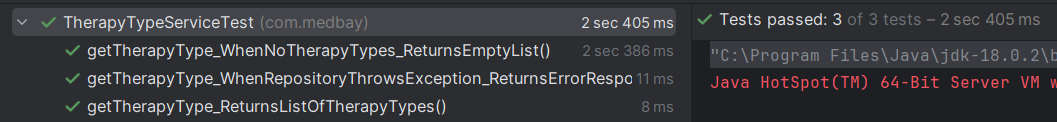
\includegraphics[width=1\linewidth]{slike/therapyTypeServiceTest.png}
				\caption{Rezultati testova za TherapyTypeService}
				\label{fig:enter-label}
			\end{figure}

			\newblock \textbf{Rezultati ispitivanja komponenti za \href{https://github.com/Project-MedBay/backend/blob/main/src/test/java/com/medbay/TherapyServiceTest.java}{TherapyService}}

			\begin{enumerate}
				\item \textbf{Test: getTherapies\_ReturnsListOfTherapies}
				\begin{itemize}
					\item \textit{Opis:} Provjera vraćanja liste terapija.
					\item \textit{Rezultat:} Test uspješan. Vraćena lista terapija.
				\end{itemize}
\begin{lstlisting}[language=Java]
@Test
void getTherapies_ReturnsListOfTherapies() {
	List<Therapy> expectedTherapies = Arrays.asList(buildTherapy("1"), buildTherapy("2"));
	when(therapyRepository.findAll()).thenReturn(expectedTherapies);
	ResponseEntity<List<Therapy>> response = therapyService.getTherapies();
	assertEquals(HttpStatus.OK, response.getStatusCode());
	assertEquals(expectedTherapies, response.getBody());
}
\end{lstlisting}
					
				\item \textbf{Test: getTherapies\_WhenNoTherapies\_ReturnsEmptyList}
				\begin{itemize}
					\item \textit{Opis:} Provjera vraćanja prazne liste kada nema terapija.
					\item \textit{Rezultat:} Test uspješan. Vraćena prazna lista.
				\end{itemize}

\begin{lstlisting}[language=Java]
@Test
void getTherapies_WhenNoTherapies_ReturnsEmptyList() {
	when(therapyRepository.findAll()).thenReturn(Collections.emptyList());
	ResponseEntity<List<Therapy>> response = therapyService.getTherapies();
	assertEquals(HttpStatus.OK, response.StatusCode());
	assertTrue(Objects.requireNonNull(response.getBody()).isEmpty());
}
\end{lstlisting}
					
				\item \textbf{Test: deleteTherapy\_WhenTherapyExists\_DeletesTherapy}
				\begin{itemize}
					\item \textit{Opis:} Provjera brisanja postojeće terapije.
					\item \textit{Rezultat:} Test uspješan. Terapija izbrisana.
				\end{itemize}

\begin{lstlisting}[language=Java]
@Test
void deleteTherapy_WhenTherapyExists_DeletesTherapy() {
	Long therapyId = 1L;
	when(therapyRepository.existsById(therapyId)).thenReturn(true);
	ResponseEntity<Void> response = therapyService.deleteTherapy(therapyId);
	assertEquals(HttpStatus.OK, response.getStatusCode());
	verify(therapyRepository).deleteById(therapyId);
}
\end{lstlisting}
					
				\item \textbf{Test: deleteTherapy\_WhenTherapyDoesNotExist\_ReturnsNotFound}
				\begin{itemize}
					\item \textit{Opis:} Provjera odziva kada terapija ne postoji.
					\item \textit{Rezultat:} Test uspješan. Vraćen status "Nije pronađeno".
				\end{itemize}

\begin{lstlisting}[language=Java]
@Test
void deleteTherapy_WhenTherapyDoesNotExist_ReturnsNotFound() {
	Long therapyId = 1L;
	when(therapyRepository.existsById(therapyId)).thenReturn(false);
	ResponseEntity<Void> response = therapyService.deleteTherapy(therapyId);
	assertEquals(HttpStatus.NOT_FOUND, response.getStatusCode());
	verify(therapyRepository, never()).deleteById(therapyId);
}
\end{lstlisting}
					
			\end{enumerate}
			\begin{figure}[!h]
				\centering
				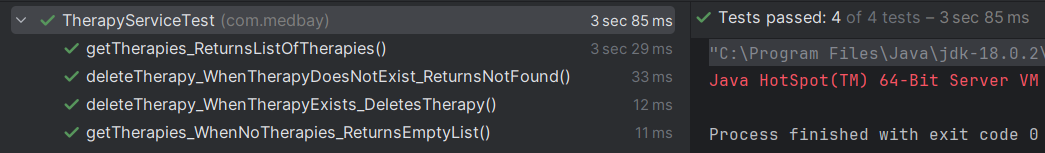
\includegraphics[width=1\linewidth]{slike/therapyServiceTest.png}
				\caption{Rezultati testova za TherapyService}
				\label{fig:enter-label}
			\end{figure}


			Svi testovi su uspješno prošli, što ukazuje na pouzdanost i ispravnost implementacije u razredu \texttt{TherapyService}. \newline

			Napomena: Prilikom klika na naziv razreda korištenih za testiranje otvara se internet poveznica na kojoj se može vidjeti izvorni kod testova.

			
			
			\subsection{Ispitivanje sustava}
			Svi testovi osim registracije i zaboravljene lozinke izvršeni su uz pomoć Selenium WebDrivera . Ispitivanje se radilo po obrascima uporabe kako bi
se provjerile funkcionalnosti sustava. Prikazivanje ispitivanja UC1, UC3, UC4, UC5, UC6, UC i UC13 (uključujući UC7).
			\newline
			\textbf{Ispitni sučaj 1: Registracija} 
			\begin{enumerate}
				\item Otvaranje stranice za registraciju.
				\item Unos obveznih podataka: ime, prezime, email, datum rođenja, adresa, broj telefona, MBO, lozinka.
				\item Riješavanje Google reCAPTCHA.
				\item Klik na gumb za registraciju.
			\end{enumerate}
			\textbf{Očekivani izlaz:}
			\begin{enumerate}
				\item Prikaz poruke o uspjehu slanja zahtjeva za registraciju.
			\end{enumerate}
			\textbf{Rezultat:} Očekivani rezultat je zadovoljen. \color{green} Aplikacija je prošla test. \color{black} \newline
			\textbf{Ispitni sučaj 2: Prijava na stranicu} 
			\textbf{Ulaz:}
			\begin{enumerate}
				\item Otvaranje početne stranice.
				\item Unos e-maila i lozinka.
				\item Klik na gumb za prijavu.
			\end{enumerate}
			\textbf{Očekivani izlaz:}
			\begin{enumerate}
				\item Uspješna prijava i preusmjeravanje na početnu stranicu za pacijente.
			\end{enumerate}
			\textbf{Rezultat:} Očekivani rezultat je zadovoljen. \color{green} Aplikacija je prošla test. \color{black} \newline
			\textbf{Ispitni slučaj 3: Promjena termina terapije}
			\begin{enumerate}
				\item Klik na prvi termin terapije.
				\item Klik na opciju "Odgodi termin".
				\item Promjena datuma termina iza posljednjeg termina terapije.
				\item Potvrda odabira i klik na gumb za potvrdu odgode.
				\item Klik na poslijednji termin terapije.
				\item Klik na opciju "Odgodi termin".
				\item Promjena datuma termina na orginalni datum.
				\item Potvrda odabira i klik na gumb za potvrdu odgode.
			\end{enumerate}
			\textbf{Očekivani izlaz:}
			\begin{enumerate}
				\item[1.a] Uspješna promjena datuma termina.
				\item[1.b] Informacije o terminu promijenjene i odgovaraju novom datumu.
				\item[2.a] Uspješna promjena datuma termina.
				\item[2.b] Informacije o terminu promijenjene i odgovaraju novom datumu.
			\end{enumerate}
			\textbf{Rezultat:} Očekivani rezultat [2.b] nije zadovoljen jer se redni broj termina prikazuje kao posljednji umjesto kao prvi, iako je u kalendaru na točnoj poziciji. Ostala očekivanja su zadovoljena. \color{red} Aplikacija nije prošla test. \color{black} \newline
			\textbf{Ispitni slučaj 4: Stvaranje novog zahtjeva za terapiju}
			\begin{enumerate}
				\item Klik na opciju "Nova terapija".
				\item Odabir vrste terapije i unos potrebnih datuma.
				\item Unos verifikacijski podataka terapije sa uputnice.
				\item Potvrda odabira i klik na gumb za završetak.
				\item Prikaz poruke o uspješnom zahtjevu za novu terapiju.
			\end{enumerate}
			\textbf{Očekivani izlaz:}
			\begin{enumerate}
				\item Uspješno stvaranje terapije i prikaz potvrde. 
				\item Dodavanje termina u raspored korisnika.
			\end{enumerate}
			\textbf{Rezultat:} Sva očekivanja su zadovoljena. \color{green} Aplikacija je prošla test. \color{black} \newline
			\textbf{Ispitni slučaj 5: Zaboravljena lozinka}
			\begin{enumerate}
				\item Otvaranje početne stranice.
				\item Klik na "Zaboravljena lozinka".
				\item Upis e-mail adrese za oporavak lozinke.
				\item Klik na poveznicu koja je došla e-mailom.
				\item Upis i potvrda nove lozinke.
				\item Klik na gumb "Reset password".
				\item Spremanje promjena.
			\end{enumerate}
			\textbf{Očekivani izlaz:}
			\begin{enumerate}
				\item Sustav šalje elektronsku poštu s obrascem za promjenu lozinke.
				\item Nakon ispunjavanja obrasca uspješno promijenjena lozinka.
			\end{enumerate}
			\textbf{Rezultat:} Sva očekivanja su zadovoljena. \color{green} Aplikacija je prošla test. \color{black} \newline
			\textbf{Ispitni slučaj 6: Promjena bilješke o terminu pacijenta}
			\begin{enumerate}
				\item Odabir termina kojem želimo promijeniti bilješku o terminu.
				\item Klik na "Uredi".
				\item Promjena bilješke o terminu.
				\item Spremanje promjena.
			\end{enumerate}
			\textbf{Očekivani izlaz:}
			\begin{enumerate}
				\item Ažuriranje bilješke o terminu.
			\end{enumerate}
			\textbf{Rezultat:} Očekivani rezultat je ostvaren. \color{green} Aplikacija je prošla test. \color{black} \newline

			
			\eject 
		
		
		\section{Dijagram razmještaja}
			
			\textbf{\textit{dio 2. revizije}}
			
			Dijagram razmještaja opisuje topologiju sustava, fizičku arhitekturu i razmještaj programskih sustava te kako te cjeline komuniciraju. Na dijagramu imamo dva glavna čvora. Prvo imamo uređaj korisnika (PC, mobitel) preko čijeg web preglednika korisnik putem HTTPS-a dohvaća informacije iz drugog čvora, mjesta gdje je pohranjen kod aplikacije, baza podataka i gdje je upogonjena aplikacija. Riječ je o Herokuu, platformi za pogonjenje aplikacija na oblaku. Heroku funkcionira pomoću \textit{dynoa}, fleksibilnih i izoliranih kontejnera koji sadrže Linux. Naša web aplikacija koristi tri \textit{dynoa}. Na prvome se nalazi frontend dio aplikacije koji je napisan u okviru React. Druga komponenta je kontejner na kojemu se sadrži \textit{backend} dio aplikacije. Tu je najbitnija Spring aplikacija koja reagira na zahtjeve \textit{frontenda} i komunicira s bazom podataka, a prisutan je i kratki kod koji omogućuje rad AI bota na našoj aplikaciji. Tu se još nalazi i zadnji \textit{dyno}, Herokuova PostgreSQL usluga gdje se nalazi baza podataka koju aplikacija koristi. Kontejneri za \textit{frontend} i \textit{backend} komuniciraju HTTPS protokolom, a \textit{backend} i baza podataka s protokolima koje osmišlja i definira sam Heroku.

            \begin{figure}[H]
             \centering
             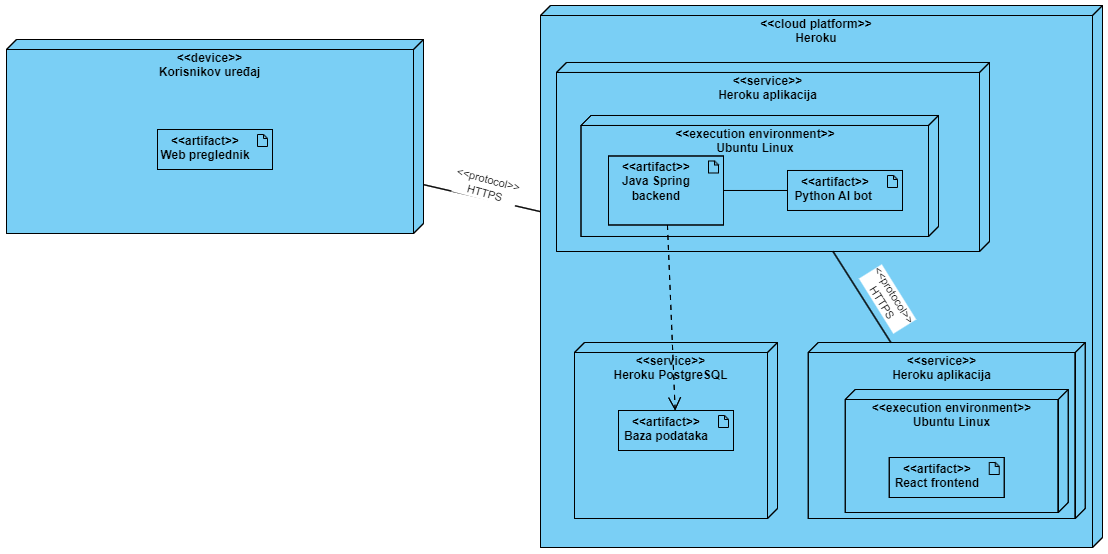
\includegraphics[width=1\linewidth]{slike/Dijagram razmjestaja.png}
             \caption{Dijagram razmještaja}
             \end{figure}
			\eject
		
		\section{Upute za puštanje u pogon}
		
		
U postavljanju i puštanju u pogon naše aplikacije ključnu ulogu igra Heroku CLI (Command Line Interface), moćan naredbeni alat koji pojednostavljuje interakciju s Heroku platformom izravno iz terminala. Instalirali smo Heroku CLI na lokalnom računalu kako bismo iskoristili njegove funkcionalnosti za upravljanje aplikacijama na Heroku platformi.

Naša integrirana strategija razvoja i puštanja u pogon koristi niz ključnih značajki Heroku platforme:

1. Automatsko puštanje u pogon s GitHub-a:
   - GitHub repozitorij povezan je s Heroku, omogućujući jednostavano automatsko puštanje u pogon naše aplikacije.
   - Svaka promjena na glavnoj grani GitHuba automatski pokreće puštanje u pogon na Heroku platformi.

2. Konfiguracijske Datoteke na Heroku:
   - Heroku nam omogućava preciznu konfiguraciju putem posebnih datoteka koje definiraju okruženje za našu aplikaciju.
   - Detaljno smo definirali parametre poput verzija jezika (Java, Python) i aktivnih profila za Spring.

3. Korištenje Financijske Potpore od Heroku:

   - Naša organizacija prima financijsku potporu od Heroku platforme, pružajući nam sredstva za korištenje resursa.


4. Baza Podataka na Heroku:
   - Integrirali smo Heroku Postgres "add-on" za potrebe baze podataka.
   - Heroku Postgres pruža siguran pristup bazama podataka putem pridruženih akreditiva.
   \begin{figure}[H]
       \centering
       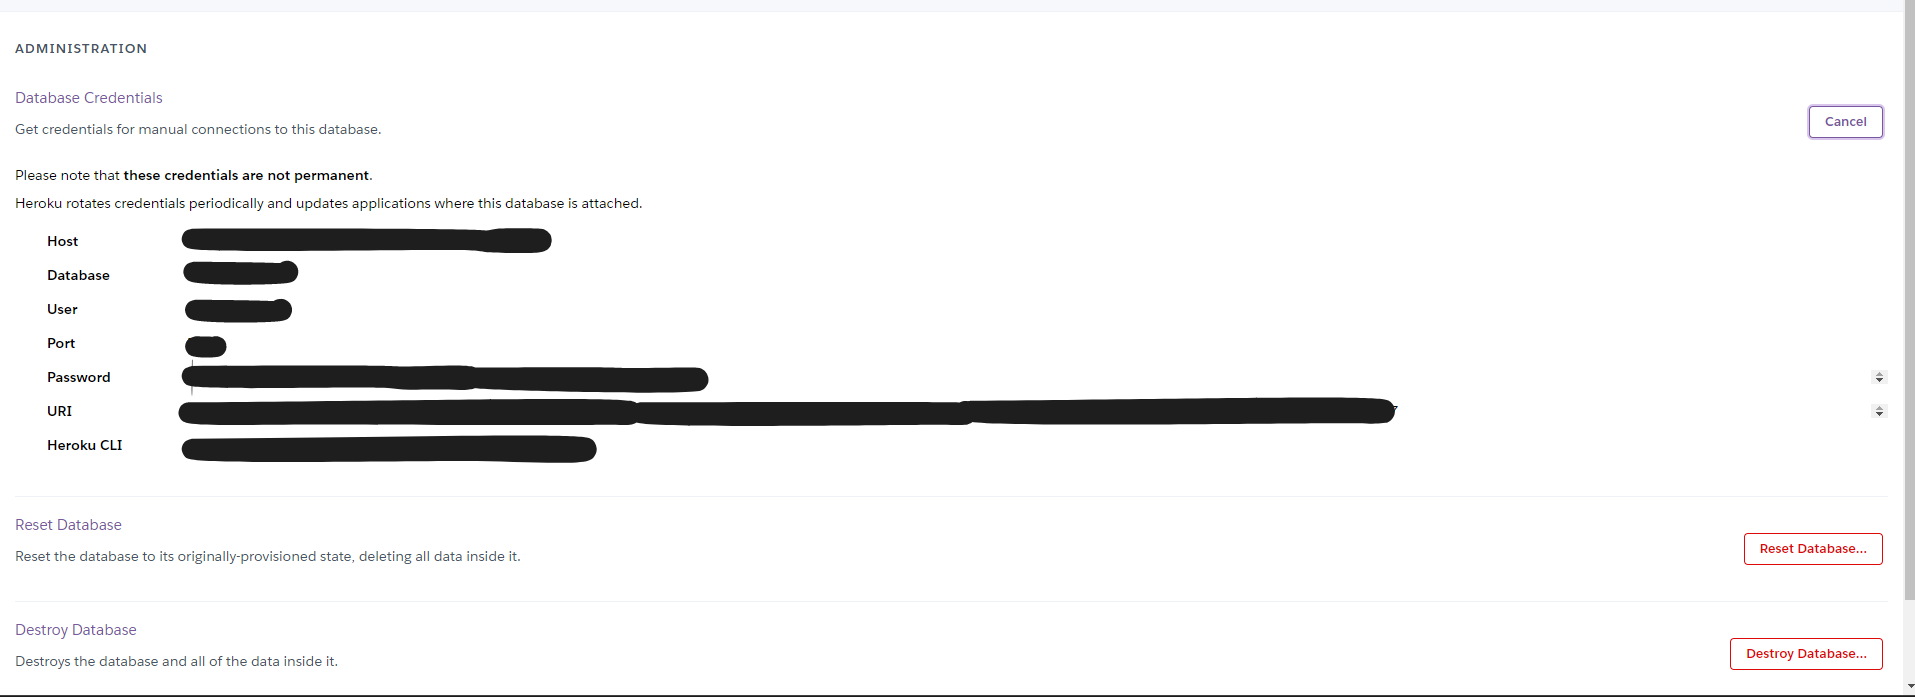
\includegraphics[width=1\linewidth]{slike/credentials.png}
       \caption{Akreditivi za našu aplikaciju}
       \label{fig:enter-label}
   \end{figure}

5. Dinamičko Okruženje s  dinamičkim kontejnerima:
   - Korištenjem dinamičkih kontejnera na Heroku stvaramo virtualno okruženje koje omogućuje izvršavanje i hostanje naše aplikacije.
   - Ime domene "medbay.life" registrirano je putem "Namecheap"-a, dok smo HTTPS certifikat dobili kroz Cloudflare za sigurnu komunikaciju.

6. Praćenje i evidentiranje:
   - Heroku pruža napredne alate za praćenje performansi, uključujući detaljne evidencije za svaki zahtjev poslan aplikaciji.
   - Metrike i analize omogućuju nam praćenje ponašanja aplikacije u stvarnom vremenu.
   \begin{figure}[H]
       \centering
       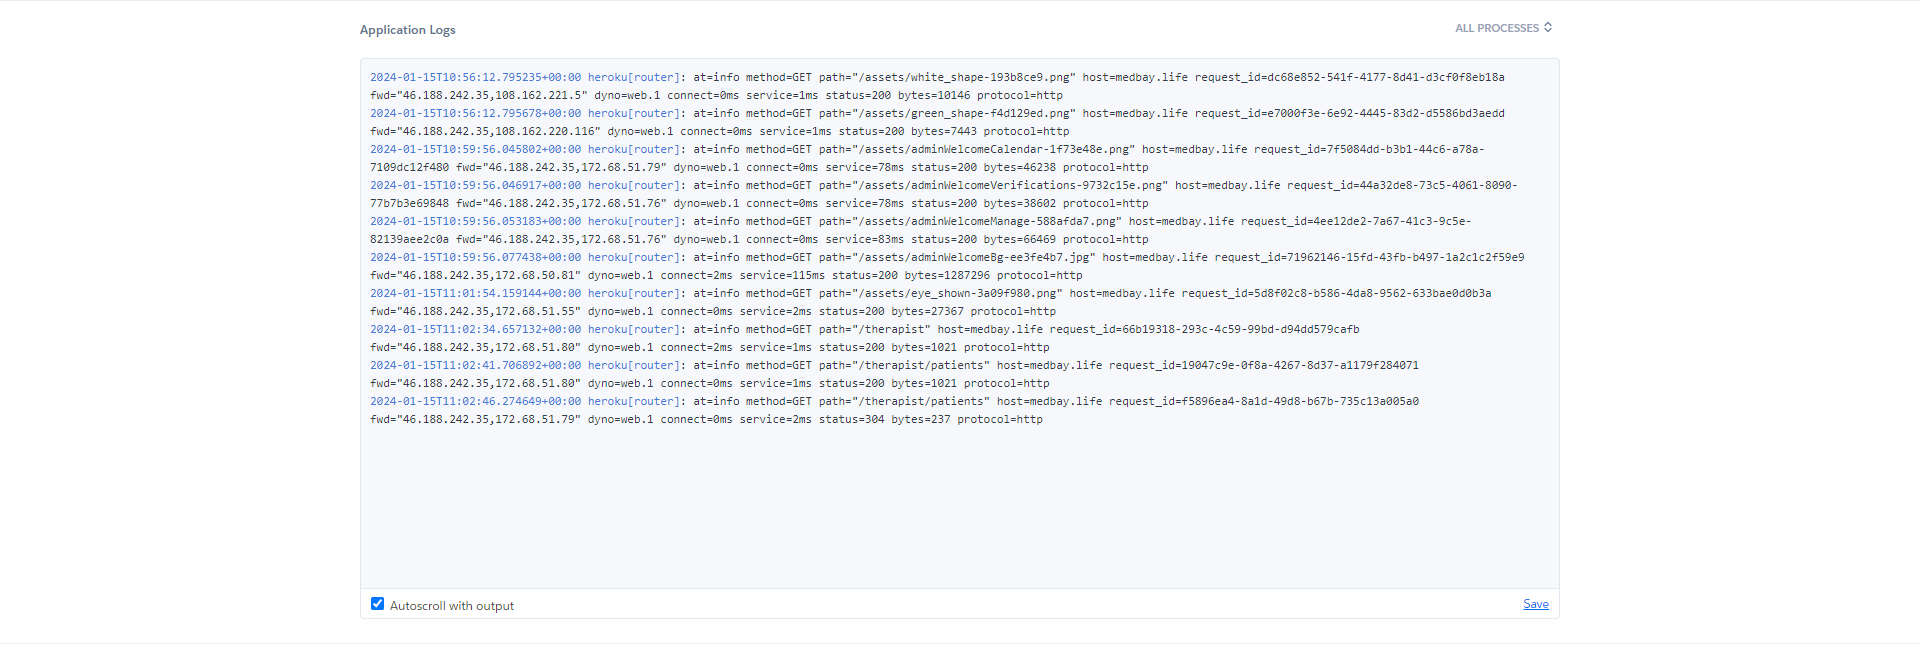
\includegraphics[width=1\linewidth]{slike/appLogs.png}
       \caption{Aplikacijsko evidentiranje}
       \label{fig:enter-label}
   \end{figure}


\begin{figure}[H]
    \centering
    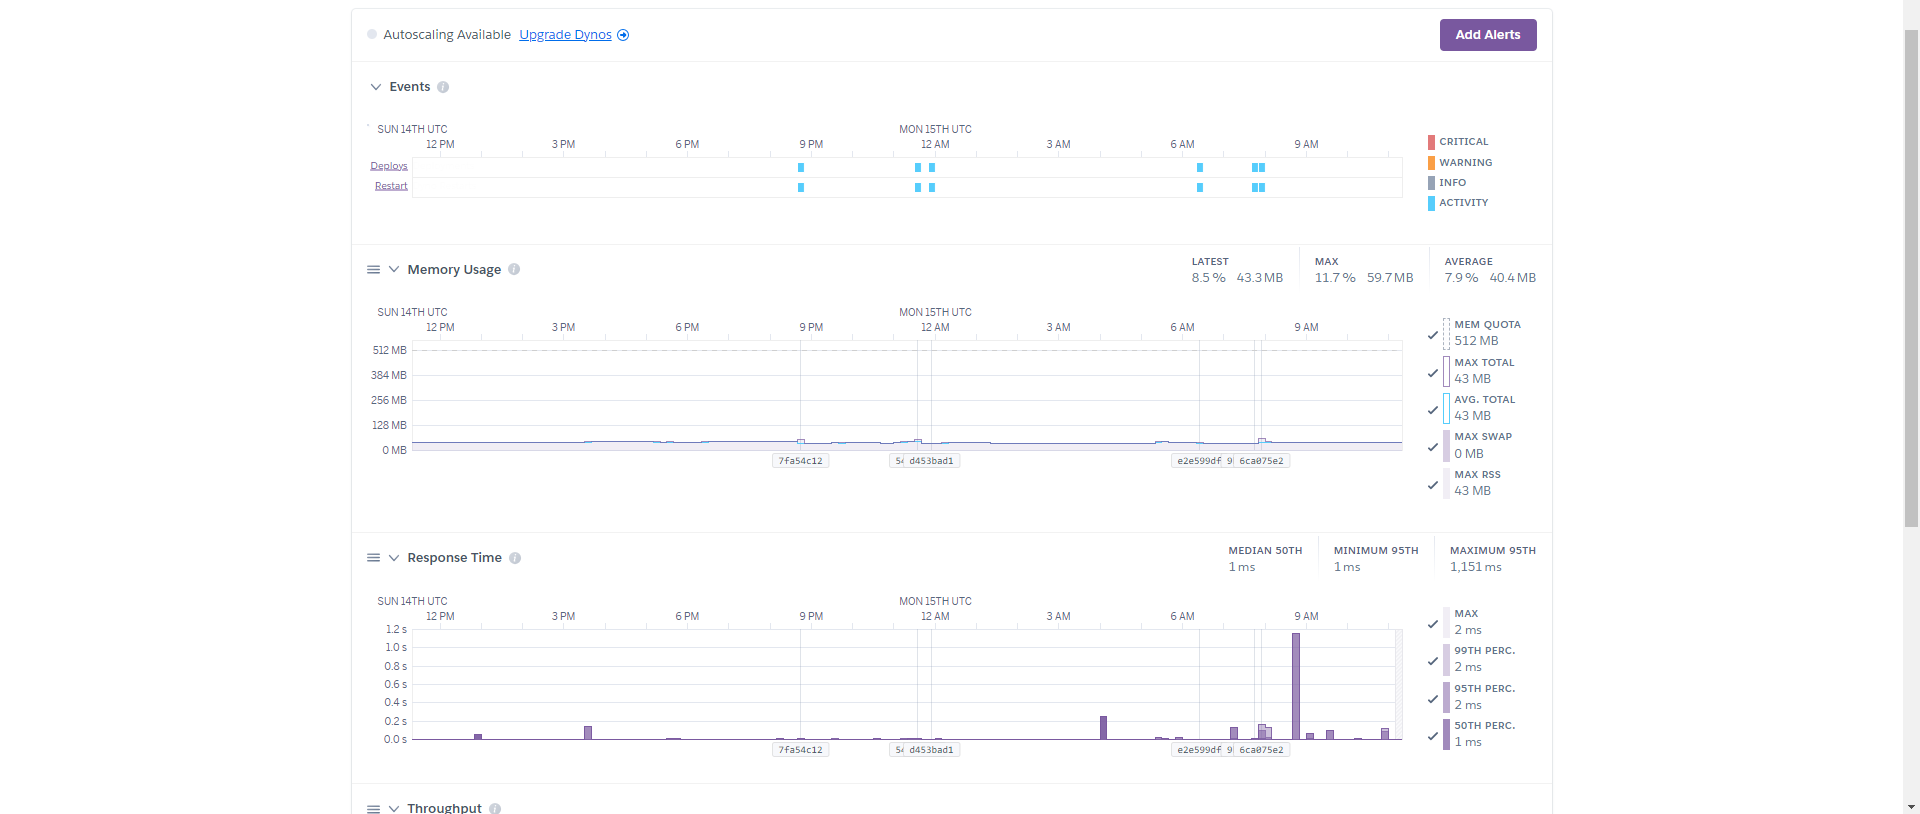
\includegraphics[width=1\linewidth]{slike/metrics.png}
    \caption{Metrika aplikacija}
    \label{fig:enter-label}
\end{figure}
7. Paketi za izgradnju:
   - Integrirali smo različite Pakete za izgradnju prilagođene jezicima koje koristimo (npr., Python, Java).
   - Automatski konfiguriraju okolinu i podržavaju različite jezične specifikacije.

Ovaj sveobuhvatan pristup omogućava nam efikasan ciklus razvoja i puštanja u pogon aplikacije. Kombinacijom GitHuba, Heroku platforme, i alata poput Heroku CLI-a, postižemo stabilan i automatski proces implementacije koji podržava dinamično okruženje naše aplikacije.


\textbf{Općenito o načinu korištenja Heroku CLI (Command Line Interface):}

1. Instalacija Heroku CLI:
   Heroku CLI smo instalirali na lokalnom računalu, omogućujući nam jednostavan pristup naredbama i funkcionalnostima koje pruža. Za instalaciju, slijedili smo upute dostupne na [službenoj Heroku stranici za instalaciju CLI-a](https://devcenter.heroku.com/articles/heroku-cli).

2. Povezivanje s Heroku Računom:
    Pomoću Heroku CLI-a uspostavili smo vezu s našim Heroku računom, omogućavajući autentikaciju i autorizaciju za izvršavanje različitih operacija. Ova faza je ključna za pristup resursima i upravljanje aplikacijom.

3. Korištenje CLI-a za puštanje u pogon aplikacije:
    Heroku CLI smo aktivno koristili za inicijalizaciju puštanje u pogon naših aplikacija. Naredbe poput `git push heroku main` omogućuju nam jednostavano i automatsko puštanje u pogon na Heroku platformu.

4. Upotreba CLI-a za Konfiguraciju Aplikacije:
    Heroku CLI pruža alate za konfiguraciju različitih aspekata aplikacije. Kroz naredbe poput `heroku config:set` postavljali smo i mijenjali okružne varijable te druge konfiguracijske postavke prema potrebama naše aplikacije.

5. Praćenje evidencija i Performansi:
    Za praćenje evidencija i performansi aplikacije koristili smo Heroku CLI. Naredbe poput `heroku logs` omogućuju nam pregled događaja u stvarnom vremenu, pružajući važne informacije o ponašanju aplikacije.

6. Dodatne Naredbe za Upravljanje Resursima:
    Heroku CLI pruža širok spektar dodatnih naredbi za upravljanje resursima. Skaliranje aplikacije, upravljanje "add-on"-ima i druge operacije mogu se jednostavno izvršiti putem ovog sučelja.

Heroku CLI je postao ključan alat u našem procesu razvoja i deploya. Omogućuje nam jednostavnu interakciju s Heroku platformom direktno iz terminala, čime poboljšavamo produktivnost i imamo veću kontrolu nad našim aplikacijama. 

